\section{Estado del arte}

En esta sección el objetivo es analizar la literatura reciente y los artículos publicados sobre el entrenamiento de modelos de aprendizaje profundo, tanto a través de técnicas basadas en gradiente descendente como metaheurísticas, enfocándonos en las familias de modelos ConvNets y MLP. Para un mejor contexto, vamos a realizar una búsqueda en la base de datos de referencias bibliográficas y citas SCOPUS, con el fin de conocer el estado actual de la literatura. Para ello la primera búsqeuda que usaremos será simple para conocer de manera general sobre el entrenamiento de modelos de aprendizaje profundo:


\begin{verbatim}

TITLE-ABS-KEY ( deep  AND learning  AND training )
AND ( LIMIT-TO ( SUBJAREA ,  "COMP" ) ) 

\end{verbatim}

El total de artículos para esta búsqueda asciende a 78.378 resultados pueden apreciarse en la figura \ref{fig:scopus_deep}. En ella se aprecia un punto de inflexión en el año 2012, en el que empiezan a crecer las publicaciones anuales de manera exponencial, siendo estas prácticamente nulas previamente. Este año es en el que AlexNet consigue ganar la competición de ImageNet, con un aumento muy significativo del interés por las redes neuronales profundas a partir de entonces. 

\begin{figure}
    \centering
    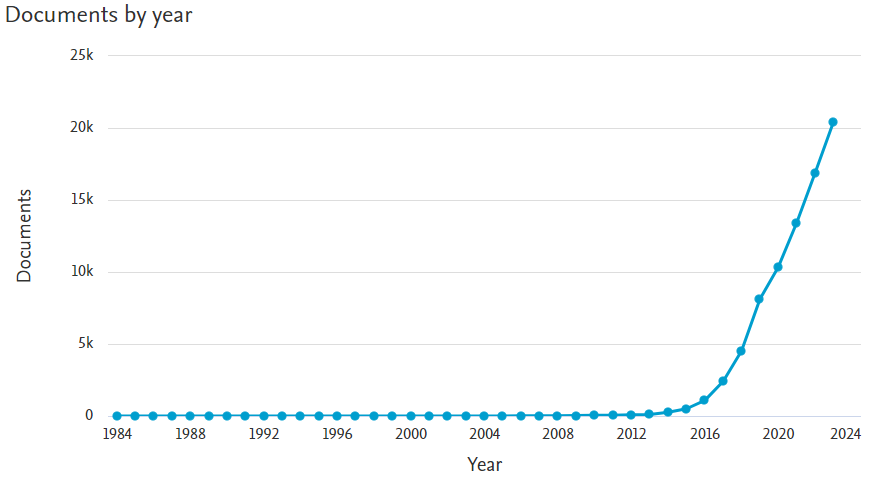
\includegraphics[width=0.75\linewidth]{Plantilla_TFG_latex//imagenes//Inf//EdA/scopus_deep.png}
    \caption{Resultados de la web SCOPUS para la búsqueda TITLE-ABS-KEY ( deep  AND learning  AND training ), muestra el número de artículos por año.}
    \label{fig:scopus_deep}
\end{figure}


Ahora vamos a realizar una búsqueda en el ámbito del entrenamiento de modelos de aprendizaje profundo pero diferenciando entre las técnicas clásicas y las técnicas metaheurísticas, para ello se usan los términos definitorios además de los nombres de las técnicas que se emplean en este TFG, realizando las siguientes búsquedas:

\begin{verbatim}
	TITLE-ABS-KEY ( ( deep  AND  learning )  AND  training  AND 
	( metaheuristic  OR  metaheuristics  OR  shade  OR  shade-ils 
	OR  ( differential  AND  evolution )  OR  memetic  OR 
	genetic ) )  AND  ( LIMIT-TO ( SUBJAREA ,  "COMP" ) )

\end{verbatim}

\begin{verbatim}
	TITLE-ABS-KEY ( ( deep  AND  learning )  AND  training  AND 
	( gradient  OR  adam  OR  optimizer  OR  rmsprop  OR  nag ) )  
	AND  ( LIMIT-TO ( SUBJAREA ,  "COMP" ) ) 
\end{verbatim}

\begin{figure}[!tbp]
\label{fig:resEdA}
  \centering
  \subfloat{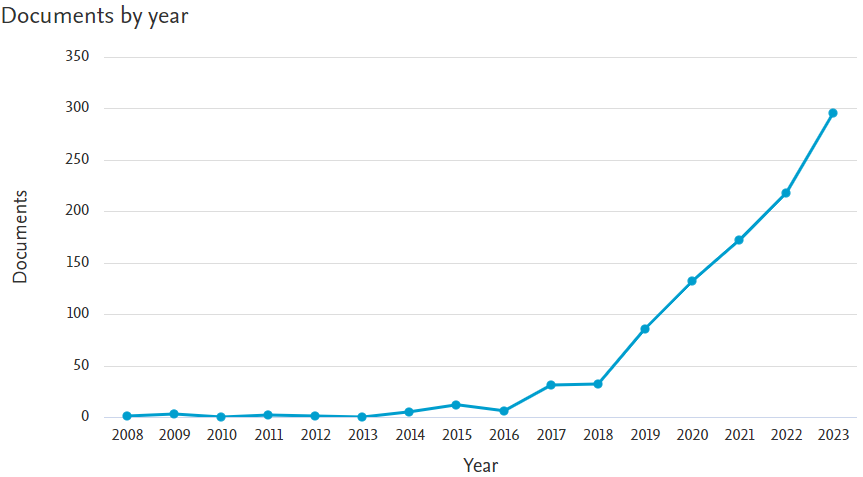
\includegraphics[width=0.75\textwidth]{Plantilla_TFG_latex//imagenes//Inf//EdA/scopus_mh.png}}
  \hfill
  \subfloat{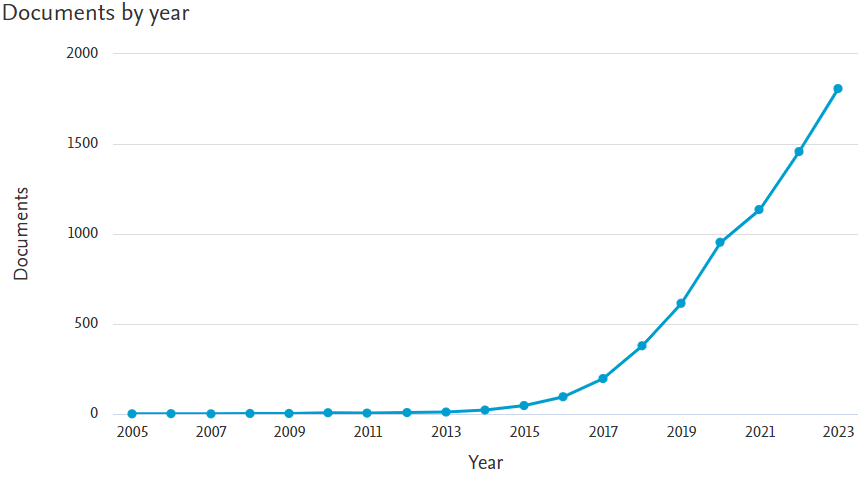
\includegraphics[width=0.75\textwidth]{Plantilla_TFG_latex//imagenes//Inf//EdA/scopus_gd.png}}
  \caption{Artículos publicados por año para el entrenamiento de modelos de aprendizaje profundo con metaheurísticas (arriba) y gradiente descendente (debajo) según las búsquedas correspondientes.}
\end{figure}

Obtenemos una cantidad de 6753 artículos en lo referente al entrenamiento de modelos de aprendizaje profundo con técnicas basadas en gradiente descendente y 997 para técnicas metaheurísticas. Vemos que la diferencia entre ambas cantidades es grande, siendo la primera 7 veces mayor que la segunda. Destacamos sin embargo que la tendencia en ambos casos es muy similar, como se observa en la figura \ref{fig:resEdA} aumentando prácticamente en la misma proporción desde el año 2012.



\subsection{Gradiente descendente y optimizadores}

El gradiente descendente es el algoritmo de aprendizaje usado por defecto prácticamente en la totalidad de los modelos de aprendizaje profundo gracias a su eficiencia y buenos resultados. Los problemas que aparecen en su convergencia se buscan evitar en la práctica a través del desarrollo de modificaciones a su algoritmo llamadas optimizadores. La literatura en este sentido es extensa, existiendo multitud de optimizadores. Primero vamos a hacer una distinción clara entre optimizadores de primer y de segundo orden. 

Aunque los de segundo orden tienen mejores propiedades teóricas y proporcionan una convergencia más rápida y más estable, ya que usan más información del problema, el hecho de tener que calcular o aproximar la matriz Hessiana aumenta demasiado el poder computacional que se requiere para utilizarlos, ralentizando mucho el entrenamiento. También hay un problema de memoria, ya que para una red neuronal de 1 millón de parámetros se necesitaría almacenar una matriz de tamaño [1.000.000, 1.000.000], ocupando aproximadamente unos 3725GB de memoria RAM. Esto resulta inabarcable más aún viendo que en el top-10 modelos de clasificación de ImageNet ningún modelo baja de los mil millones de parámetros. 

Incluso si eliminamos estos inconvenientes de memoria con métodos como L-BFGS (ver sección \ref{sec:l-bfgs}, tenemos un gran inconveniente con él y es que debemos hacer el cálculo sobre todo el conjunto de entrenamiento. Estos pueden contener del orden de millones de ejemplos (ImageNet tiene más de un millón), haciendo su cálculo inasequible computacionalmente. Conseguir que este tipo de algoritmos como L-BFGS funcionen con mini-batches es más complejo que en MBGD y de hecho es un área abierta de investigación.

En la práctica no es común ver L-BFGS u otros optimizadores de segundo orden aplicados a modelos de apendizaje profundo a gran escala. En su lugar se utilizan variantes de MBGD basadas en el uso de momento y en learning rates adaptativos ya que son mucho más simples y más escalables. Existen varias opciones bastante asentadas, que forman parte de las librerías de aprendizaje automático más usadas como PyTorch y TensorFlow, que son Adam, NAG, RMSProp, AdaGrad o SGD con momento, entre otras. Para atender a las técnicas más novedosas que alcanzan un rendimiento del estado del arte, vamos a analizar la siguiente comparativa: https://akyrillidis.github.io/2020/03/05/algo.html. 

En él se hace una comparativa de varios algoritmos con learning rate adaptativo (Adam, AMSGrad, AdamW, QHAdam, Demon Adam) y con learning rate no adaptativo (SGDM, AggMo, QHM, Demon SGDM). Los modelos y datasets usados en este análisis pueden observarse en la tabla \ref{table:exp}. Una consideración muy importante que se realiza en dicha comparativa y que es bien sabida en el campo del aprendizaje automático es que el rendimiento de una técnica de entrenamiento está muy ligado al dominio específico del problema (UNIR ESTO A USAR EL MISMO OPT EN GD QUE MH), y puede ocurrir que un método que no sea de los mejores en términos generales sea el mejor en un problema específico. Pasamos ahora a describir rápidamente las técnicas más interesantes.

\begin{table}[]
\centering
\begin{tabular}{|c|c|}
\hline
\textbf{Dataset} & \textbf{Modelo}  \\ \hline
CIFAR10          & ResNet18         \\
CIFAR100         & VGG16            \\
STL10            & Wide ResNet 16-8 \\
FMINST           & CAPS             \\
PTB              & LSTM             \\
MNIST            & VAE              \\ \hline
\end{tabular}
\caption{Tabla con los datasets utilizados con sus respectivos modelos en la experimentación de la comparativa (enlace)}
\label{table:exp}
\end{table}

YellowFin \cite{yellowfin} es un optimizador con learning rate y momento adaptativo, de manera que mantiene dichos hiperparámetros en un intervalo donde el ratio de convergencia es una constante igual a la raíz del momento. AdamW es una extensión de adam en la que se utiliza penalización en los pesos del modelo de manera que exista un sesgo hacia valores más pequeños durante el entrenamiento, ya que normalmente se asocian valores grandes en los parámetros con el sobreajuste. Aunque Adam ya incorpora esto, AdamW realiza una pequeña modificación a través de desacoplar esta penalización a la actualización del gradiente, resultando en un impacto notable. QHADAM, DEMON ADAM, DEMON MOMENTUM, QHM, AGGMO.


Como conclusión, y atendiendo siempre al dominio específico del problema, se tiene que YellowFin es la mejor opción en caso de no disponer de recursos para ajustar los hiperparámetros, ya que adapta el momento y el learning rate a lo largo del aprendizaje. Si se dispone de recursos pero no demasiados, lo mejor son algoritmos de learning rate adaptativo de manera que sólo se tenga que ajustar el valor del momento, en concreto destacan AdamW, QHAdam y Demon Adam. En cambio si se quiere obtener el mejor rendimiento a toda costa, invirtiendo muchos recursos en el ajuste de parámteros, usar MBGD con momento es la mejor opción, aunque sea un método más clásico. En concreto se recomienda su uso con Demon.


\subsection{Metaheurísticas en el entrenamiento de modelos}

Aún con el uso de optimizadores, hay ciertos inconvenientes en el entrenamiento que están provocados por el uso de BP como método de cálculo del gradiente, o directamente al uso del gradiente y no a cómo se usa. Los más comunes son el desvanecimiento y explosión del gradiente y la tendencia a quedarse atascado en mínimos locales. Las técnicas metaheurísticas son una gran alternativa ya que sus operadores de búsqueda no dependen de BP evitando así sus problemas. 

Uno de los enfoques de aplicación de estas técnicas es la combinación con las técnicas clásicas, con diferentes aproximaciones. Por ejemplo en \cite{162} se usa el algoritmo \textit{Artificial Bee Colony} \cite{beesalgo} sobre un conjunto de soluciones aleatorias para generar un conjunto de soluciones al que aplicar el algoritmo de gradiente descendente. En \cite{155} se combina un algoritmo genético con el gradiente descendente, de manera que las nuevas soluciones son generadas con el operador de búsqueda del primero pero son evaluadas tras realizar varias épocas con el segundo. De manera similar en \cite{163} se usa la técnica metaheurística \textit{Particle Swarm Optimization} \cite{pso} para entrenar los parámetros de la última capa de una ConvNet, mientras que el resto se entrenan a través del algoritmo de gradiente descendente. La comparación arroja que la hibridación de ambas técnicas alcanza mejores resultados en términos de rapidez de convergencia y de \textit{accuracy}. Prácticamente la totalidad de la literatura referente a esta estrategia está centrada en ConvNets.

El otro enfoque es entrenar el modelo usando exclusivament algoritmos bio-inspirados. En este ámbito destacan los estudios \cite{174} y \cite{176} en los que se proponen dos técnicas basadas en \textit{Simulated Annealing} \cite{siman} para entrenar los parámetros de una ConvNet, consiguiendo mejor rendimiento y mejor velocidad de convergencia que en el mismo modelo entrenado mediante el algoritmo de gradiente descendente. Al igual que ocurre con el enfoque anterior, la gran mayoría de estos estudios están centrados en ConvNets y RNNs. 

Algo importante a destacar en lo referente a la literatura de entrenamiento de modelos con técnicas metaheurísticas es la falta de rigor y de un marco común en los estudios, de manera que no pueden realizarse comparaciones objetivas entre ellos. Estos detalles, que se comentan con más detalle en la sección \ref{sec:motinfo}, ponen en evidencia la necesidad de más experimentos bajo unas condiciones similares que permitan poder sacar conclusiones objetivas entre ellos.

El rendimiento de estas técnicas todavía no es comparable al de las técnicas clásicas. Si bien es cierto que para tareas con datasets sencillos y modelos con pocos parámetros pueden mejorar al gradiente descendente en minimizar la función de pérdida para el conjunto de entrenamiento, normalmente en generalización su rendimiento lo empeora. Para modelos con muchos parámetros el rendimiento de estas técnicas está por detrás, con resultados no muy distantes pero peores de manera general. Además hay que tener en cuenta la complejidad computacional, ya que para alcanzar un rendimiento similar al gradiente descendente estas técnicas necesitan de mucho más tiempo y recursos computacionales, por lo que no resultan una alternativa viable para este tipo de tareas.




\subsubsection{SHADE-ILS}

Presentamos ahora una de las técnicas metaheurísticas que mejor resultados ofrece actualmente en el entrenamiento de modelos. En esta sección nos limitaremos a valorar sus resultados en el trabajo \cite{MHtrainingClase}, mientras que su definición y funcionamiento se presentan en la sección \ref{sec:shade-ils}. En la experimentación de dicho trabajo se atienden tres cuestiones, las tres a través de técnicas metaheurísticas: diseño de la arquitectura, optimización de hiperparámetros y entrenamiento de los parámetros de un modelo. 

Nos centraremos en la última. Se utilizan 6 datasets distintos con diferente complejidad, y en base a ésta se elige una arquitectura de modelo concreta dentro de la familia de las ConvNets, de manera que tenga buen rendimiento en su entrenamiento a través de gradiente descendente. Se utiliza el optimizador Adam para esta tarea. En el entrenamiento con SHADE-ILS se utilizan diferentes estrategias que hacen uso de la estructura de capas de los modelos de aprendizaje profundo, realizando el entrenamiento en los pesos de diversas capas, según la estrategia, mientras se mantienen congelados los demás. También se realiza el entrenamiento de todo el modelo a la vez.

Los resultados de la experimentación son claros: solo en uno de las 6 tareas uno de los modelos entrenado con SHADE-ILS minimiza más la función de pérdida que el modelo entrenado con gradiente descendente. Además, en todos los casos, el error de test es mayor. Cabe mencionar que la generalización en los modelos es bastante buena, manteniéndose estos errores en valores cercanos a los que se obtiene en el entrenamiento, y aumentando el error en proporciones similares al modelo entrenado con Adam.


